\begin{frame}
    \centering

    \Huge
    Game Theory

    \pause
    \vspace{1.5cm}
    \normalsize
    \begin{itemize}
        \centering
        \item Players \(\hspace{1.3cm}\)
        \item Strategies \(\hspace{0.82cm}\)
        \item Payoffs/Utilities
    \end{itemize}
\end{frame}


\begin{frame}
    \frametitle{Rock-Paper-Scissors}

    \hspace{3.9cm}
    \vspace{-1cm}
    
\includegraphics[width=.39\textwidth]{Bin/rock-paper-scissors.png}
    \begin{multicols}{3}
        \begin{flushright}
            
\includegraphics[width=.25\textwidth, angle=270]{Bin/rock-paper-scissors.png}
        \end{flushright}
            
        \columnbreak
 
        \begin{equation*}
            \begin{bmatrix}
                (0,0) & (1,-1) & (-1,1) \\
                & & \\
                (-1,1) & (0,0) & (1,-1) \\
                & & \\
                (1,-1) & (-1,1) & (0,0)
            \end{bmatrix}
        \end{equation*}

        \columnbreak
        \vfill
    \end{multicols}

\end{frame}


\begin{frame}
    \centering
    
    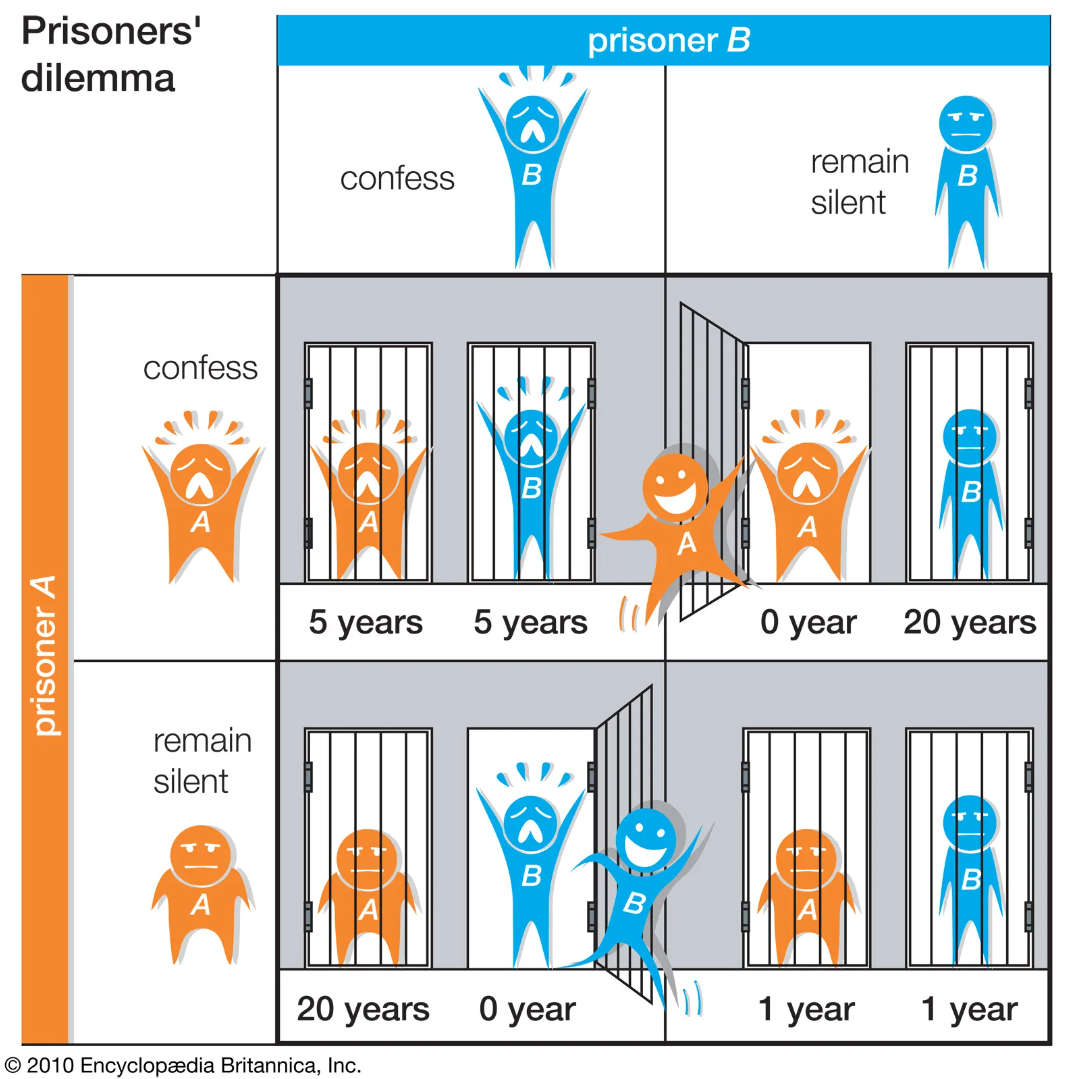
\includegraphics[height=.9\textheight]{Bin/prisonersdilemma.PNG}

\end{frame}


\begin{frame}
    \frametitle{Repeated Games}
    
    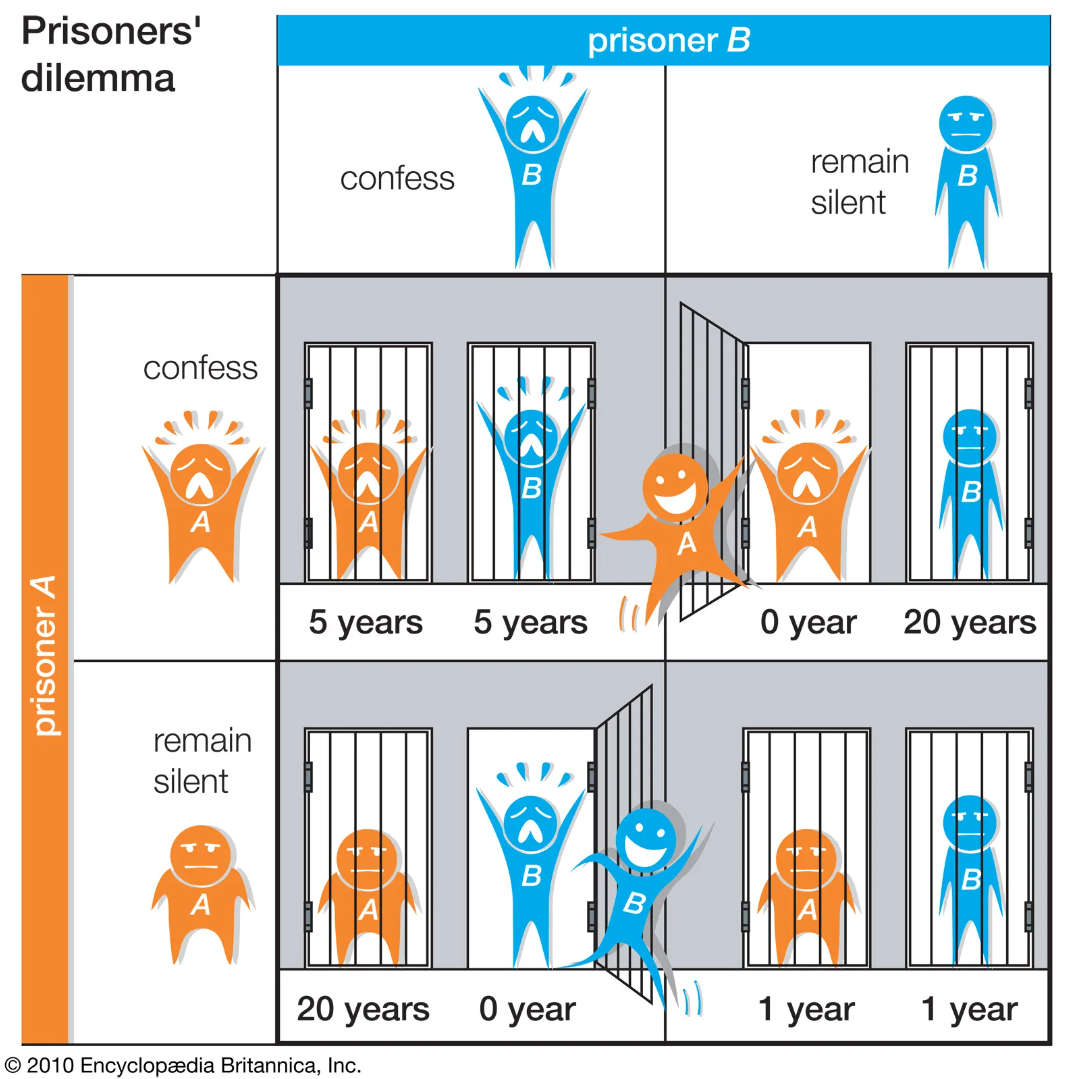
\includegraphics[width=.25\textwidth]{Bin/prisonersdilemma.PNG}
    \hspace{0.5cm}
    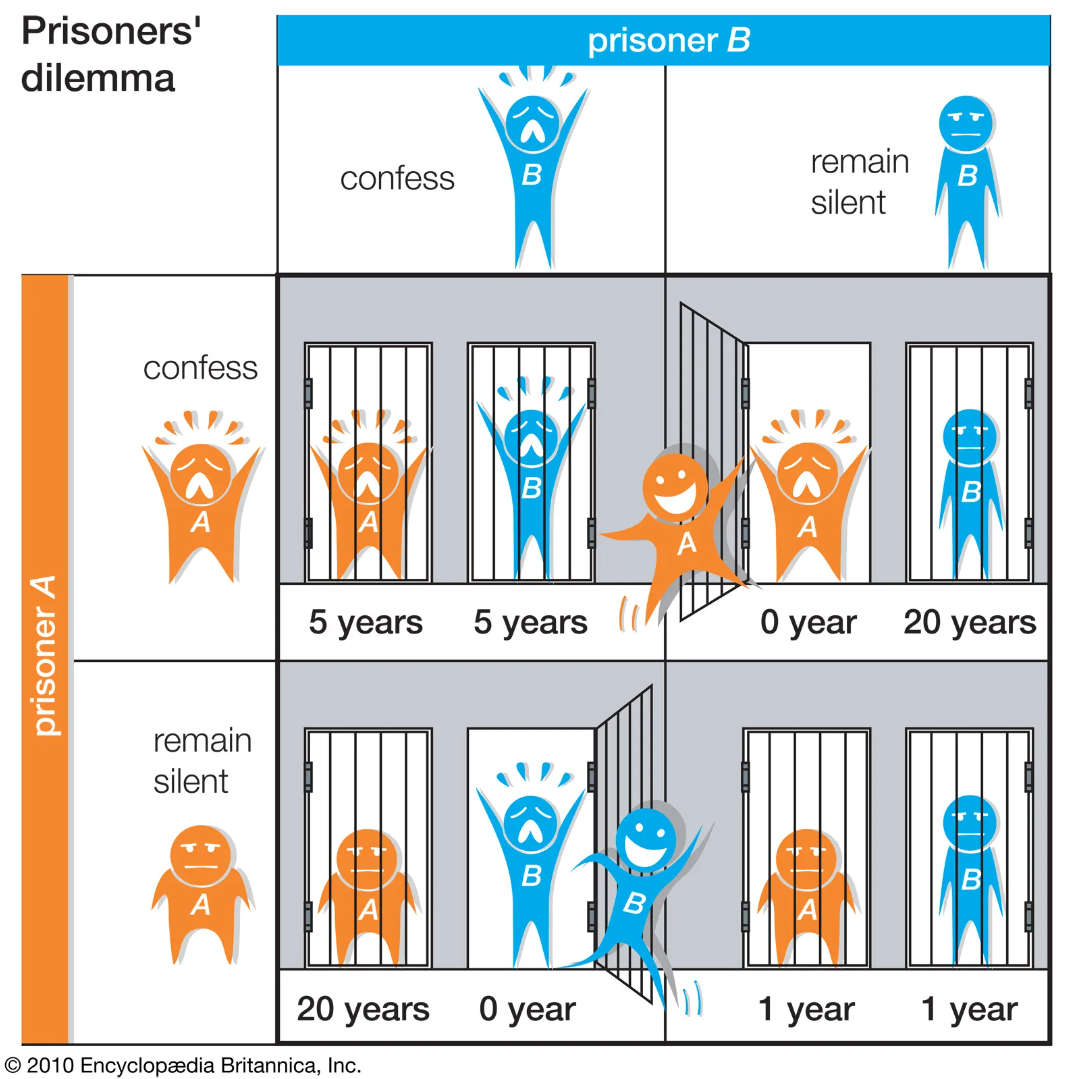
\includegraphics[width=.25\textwidth]{Bin/prisonersdilemma.PNG}
    \hspace{0.5cm}
    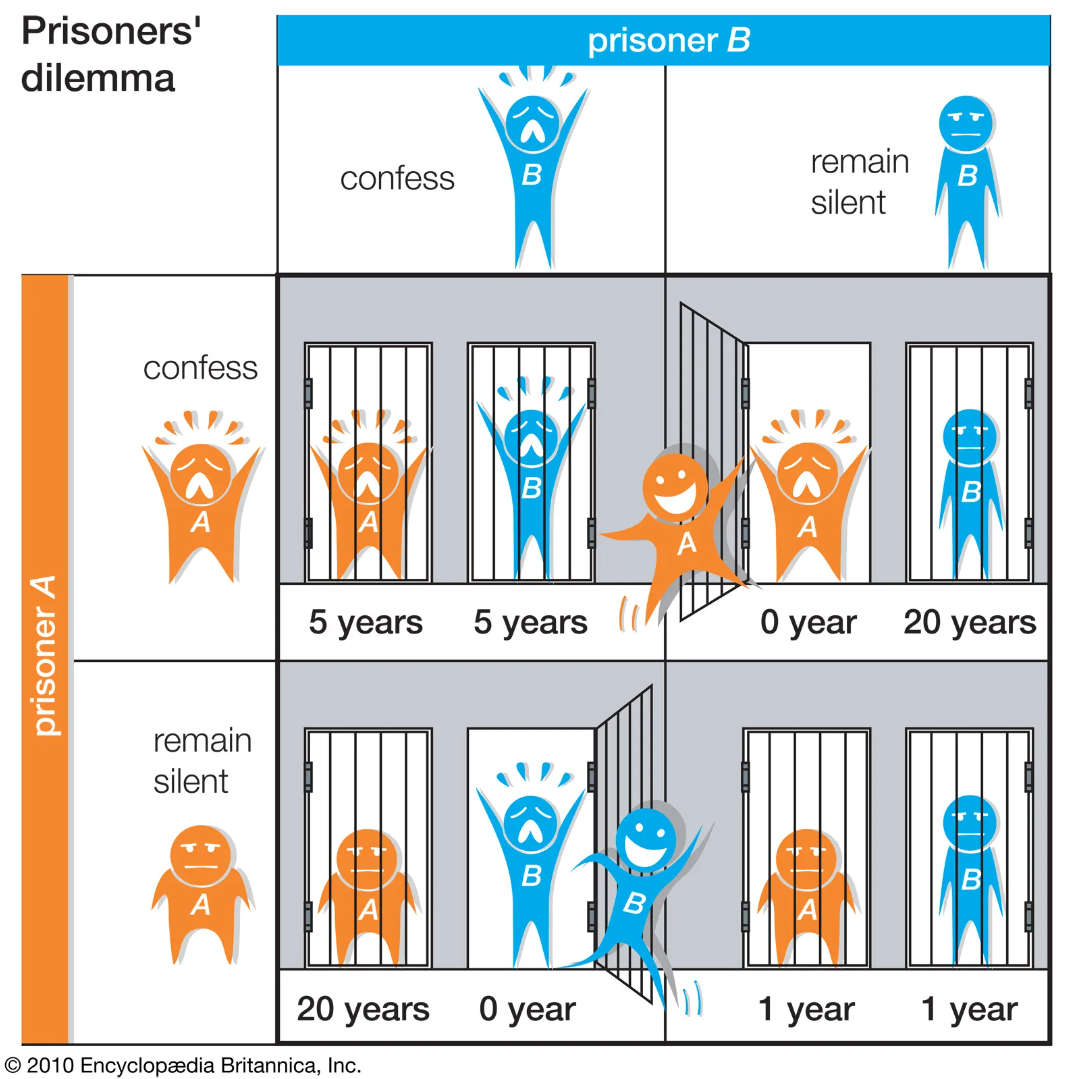
\includegraphics[width=.25\textwidth]{Bin/prisonersdilemma.PNG}

    \vspace{0.5cm}
    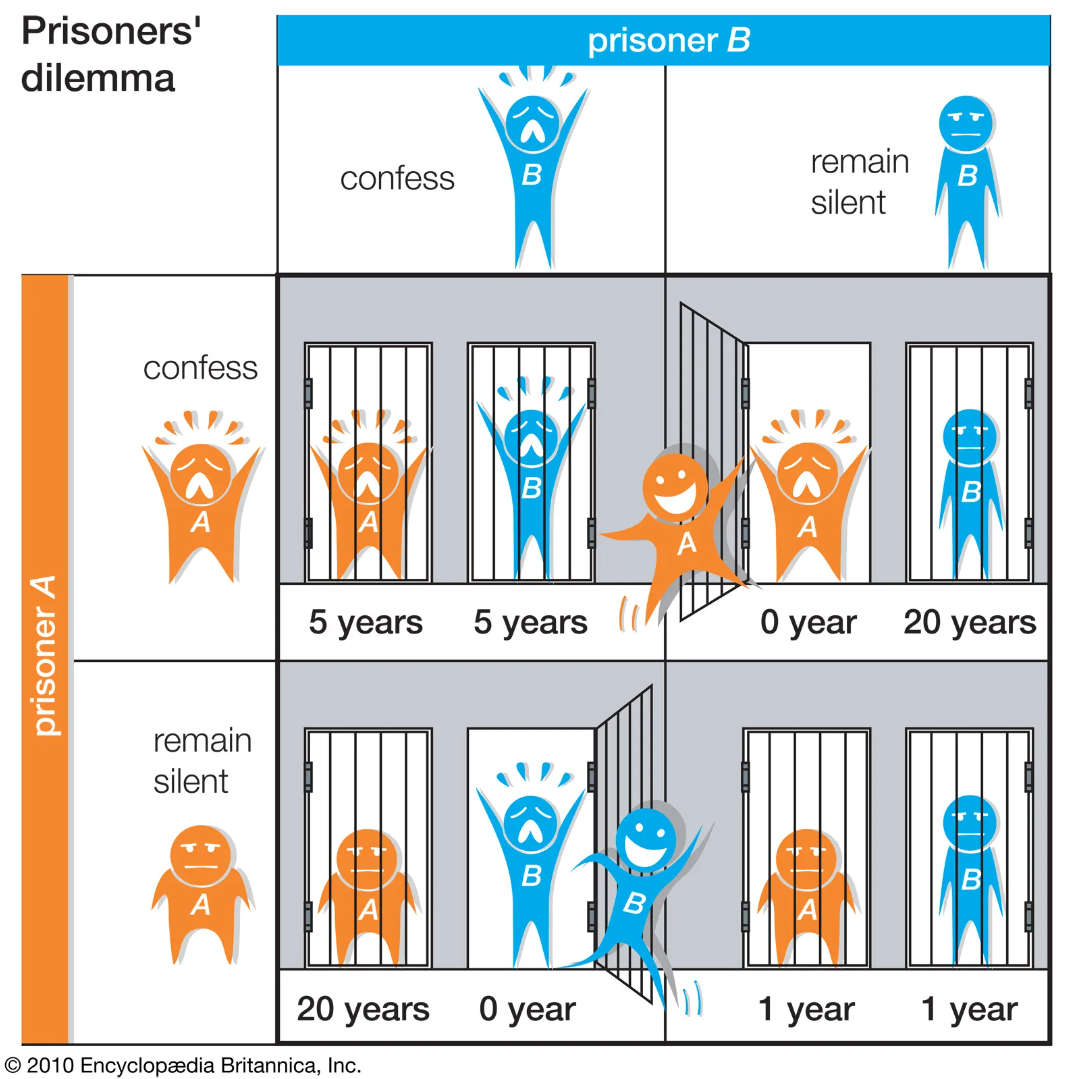
\includegraphics[width=.25\textwidth]{Bin/prisonersdilemma.PNG}
    \hspace{0.5cm}
    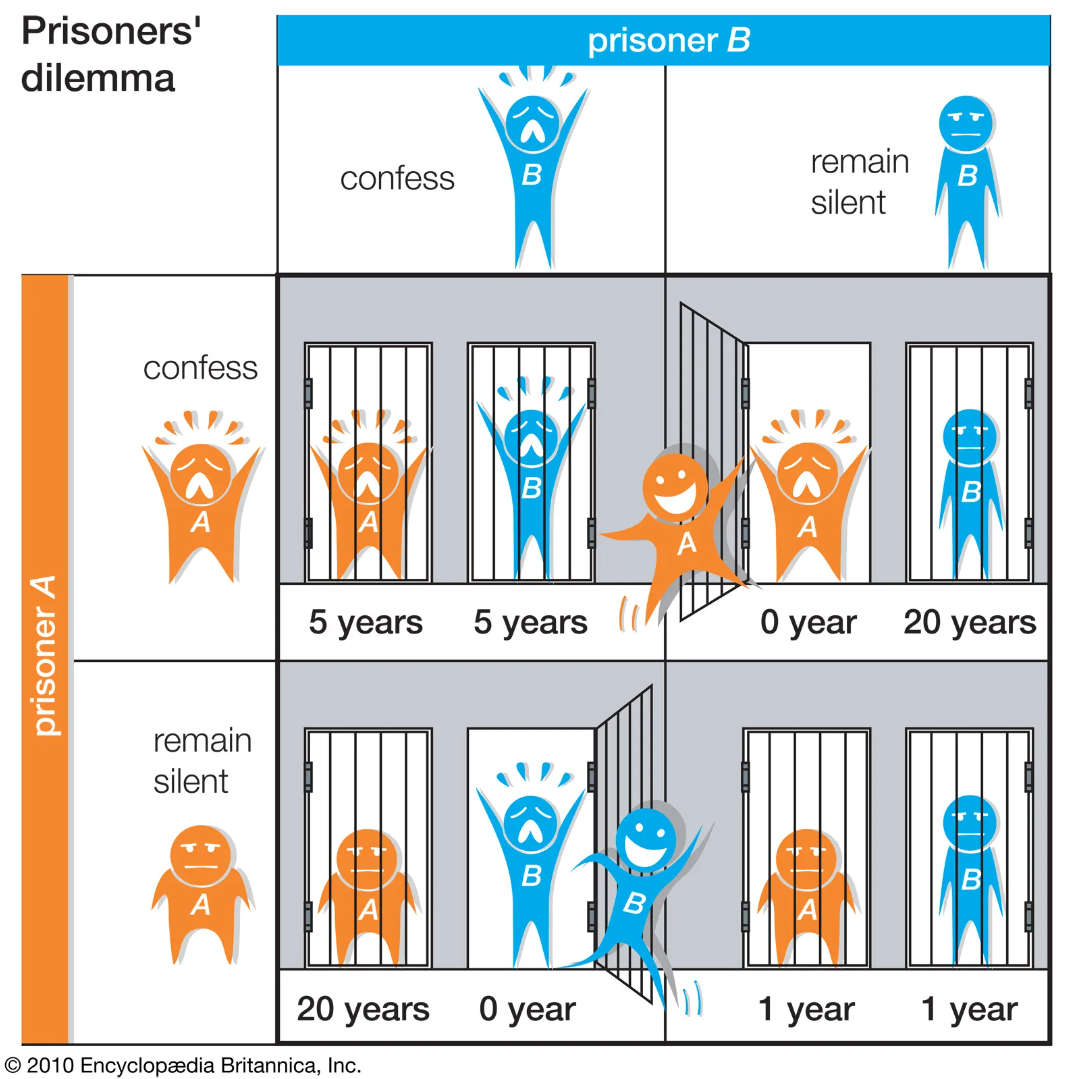
\includegraphics[width=.25\textwidth]{Bin/prisonersdilemma.PNG}
    \hspace{0.5cm}
    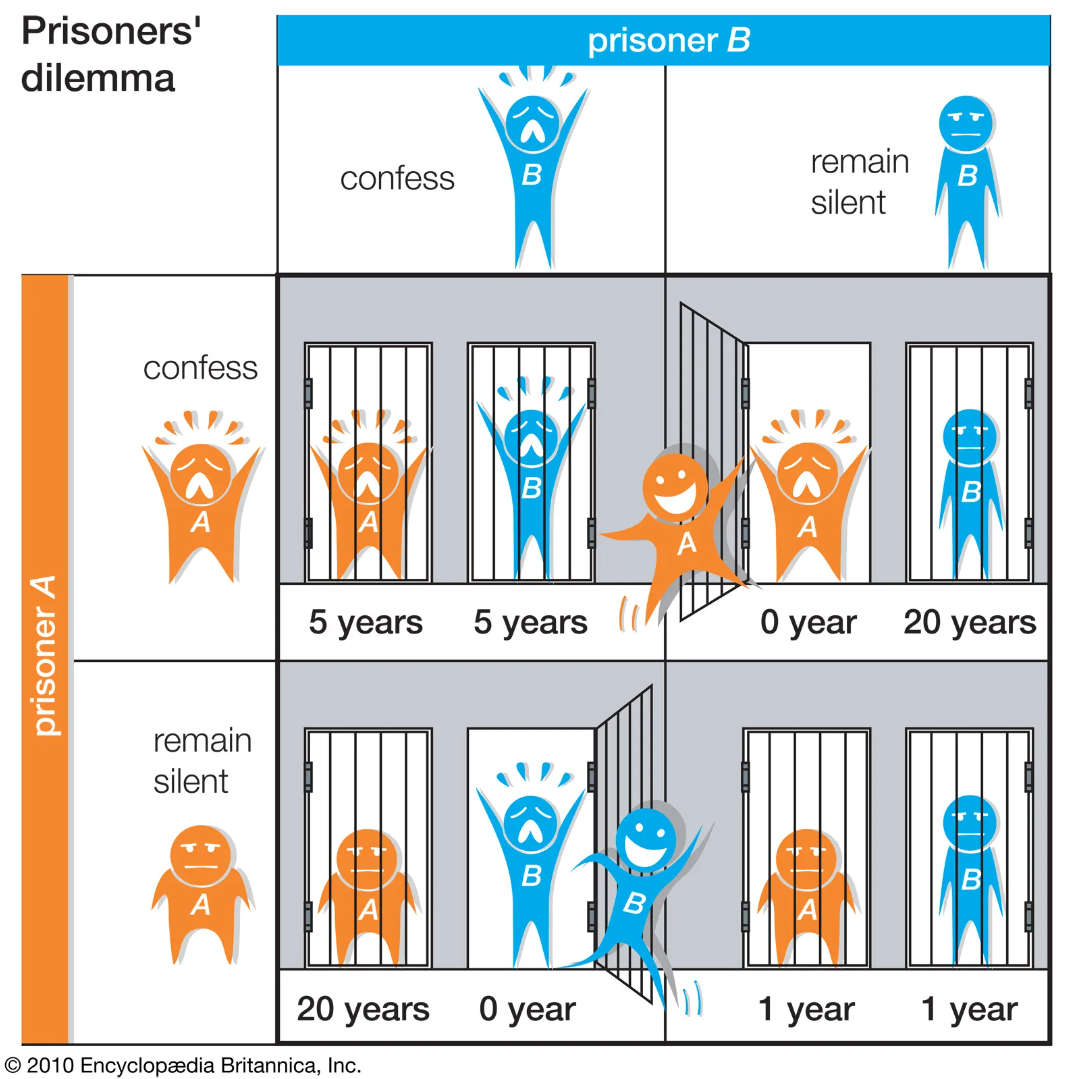
\includegraphics[width=.25\textwidth]{Bin/prisonersdilemma.PNG}

\end{frame}


\begin{frame}
    \begin{center}
        \frametitle{Prisoner's Dilemma}
        \Huge
        \begin{tabular}{|c|c|c|}
            \hline
            \diagbox{P1}{P2}    & D        & C        \\
            \hline
            D                   & \(1, 1\) & \(5, 0\) \\
            \hline
            C                   & \(0, 5\) & \(3, 3\) \\
            \hline
        \end{tabular}

        \pause
        \vspace*{1cm}
        \scriptsize
        \begin{enumerate}
            \item If both players cooperate, they both get 3 points.
            \item If both players defect, they both get 1 point.
            \item If one player defects and the other cooperates, the one that
            defects gets 5 points and the one that cooperates gets 0 points.
        \end{enumerate}
    \end{center}
\end{frame}

\begin{frame}
    \begin{center}
        \frametitle{Axelrod's Tournament - 14 strategies + 1 random}
        
        \begin{multicols}{3}
            \begin{itemize}
                \item Tit For Tat
                \item Tideman \& Chieruzzi
                \item Nydegger
                \item Grofman
                \item Shubik
                \item Stein \& Rapoport
                \item Grudger
                \item Davis
                \item Graaskamp
                \item FirstByDowning
                \item Feld
                \item Joss
                \item Tullock
                \item Unknown
                \item Random
            \end{itemize}
        \end{multicols}

    \end{center}
\end{frame}


\begin{frame}
    \frametitle{Exploring the game}
    
    \large
    \textbf{Nash equilibrium}
    \hspace{2cm}
    \textbf{Learning algorithms}

    \normalsize
    \vspace{0.5cm}
    \begin{multicols}{2}
        \begin{itemize}
            \item Lemke-Howson algorithm
            \vspace{0.5cm}
            \item Support enumeration

            \item Fictitious play
            \vspace{0.5cm}
            \item Replicator dynamics
        \end{itemize}
    \end{multicols}
\end{frame}


\begin{frame}
    \frametitle{Replicator Dynamics - Driving on the Left game}
    \centering
    \Large
    \vspace{0.5cm}
    \begin{tabular}{|c|c|c|}
        \hline
        & R  & L \\
        \hline
        R & \(1\) & \(-1\) \\
        \hline
        L & \(-1\) & \(1\) \\
        \hline
    \end{tabular}
    \vspace{0.5cm}
    \pause
    \only<2>{
        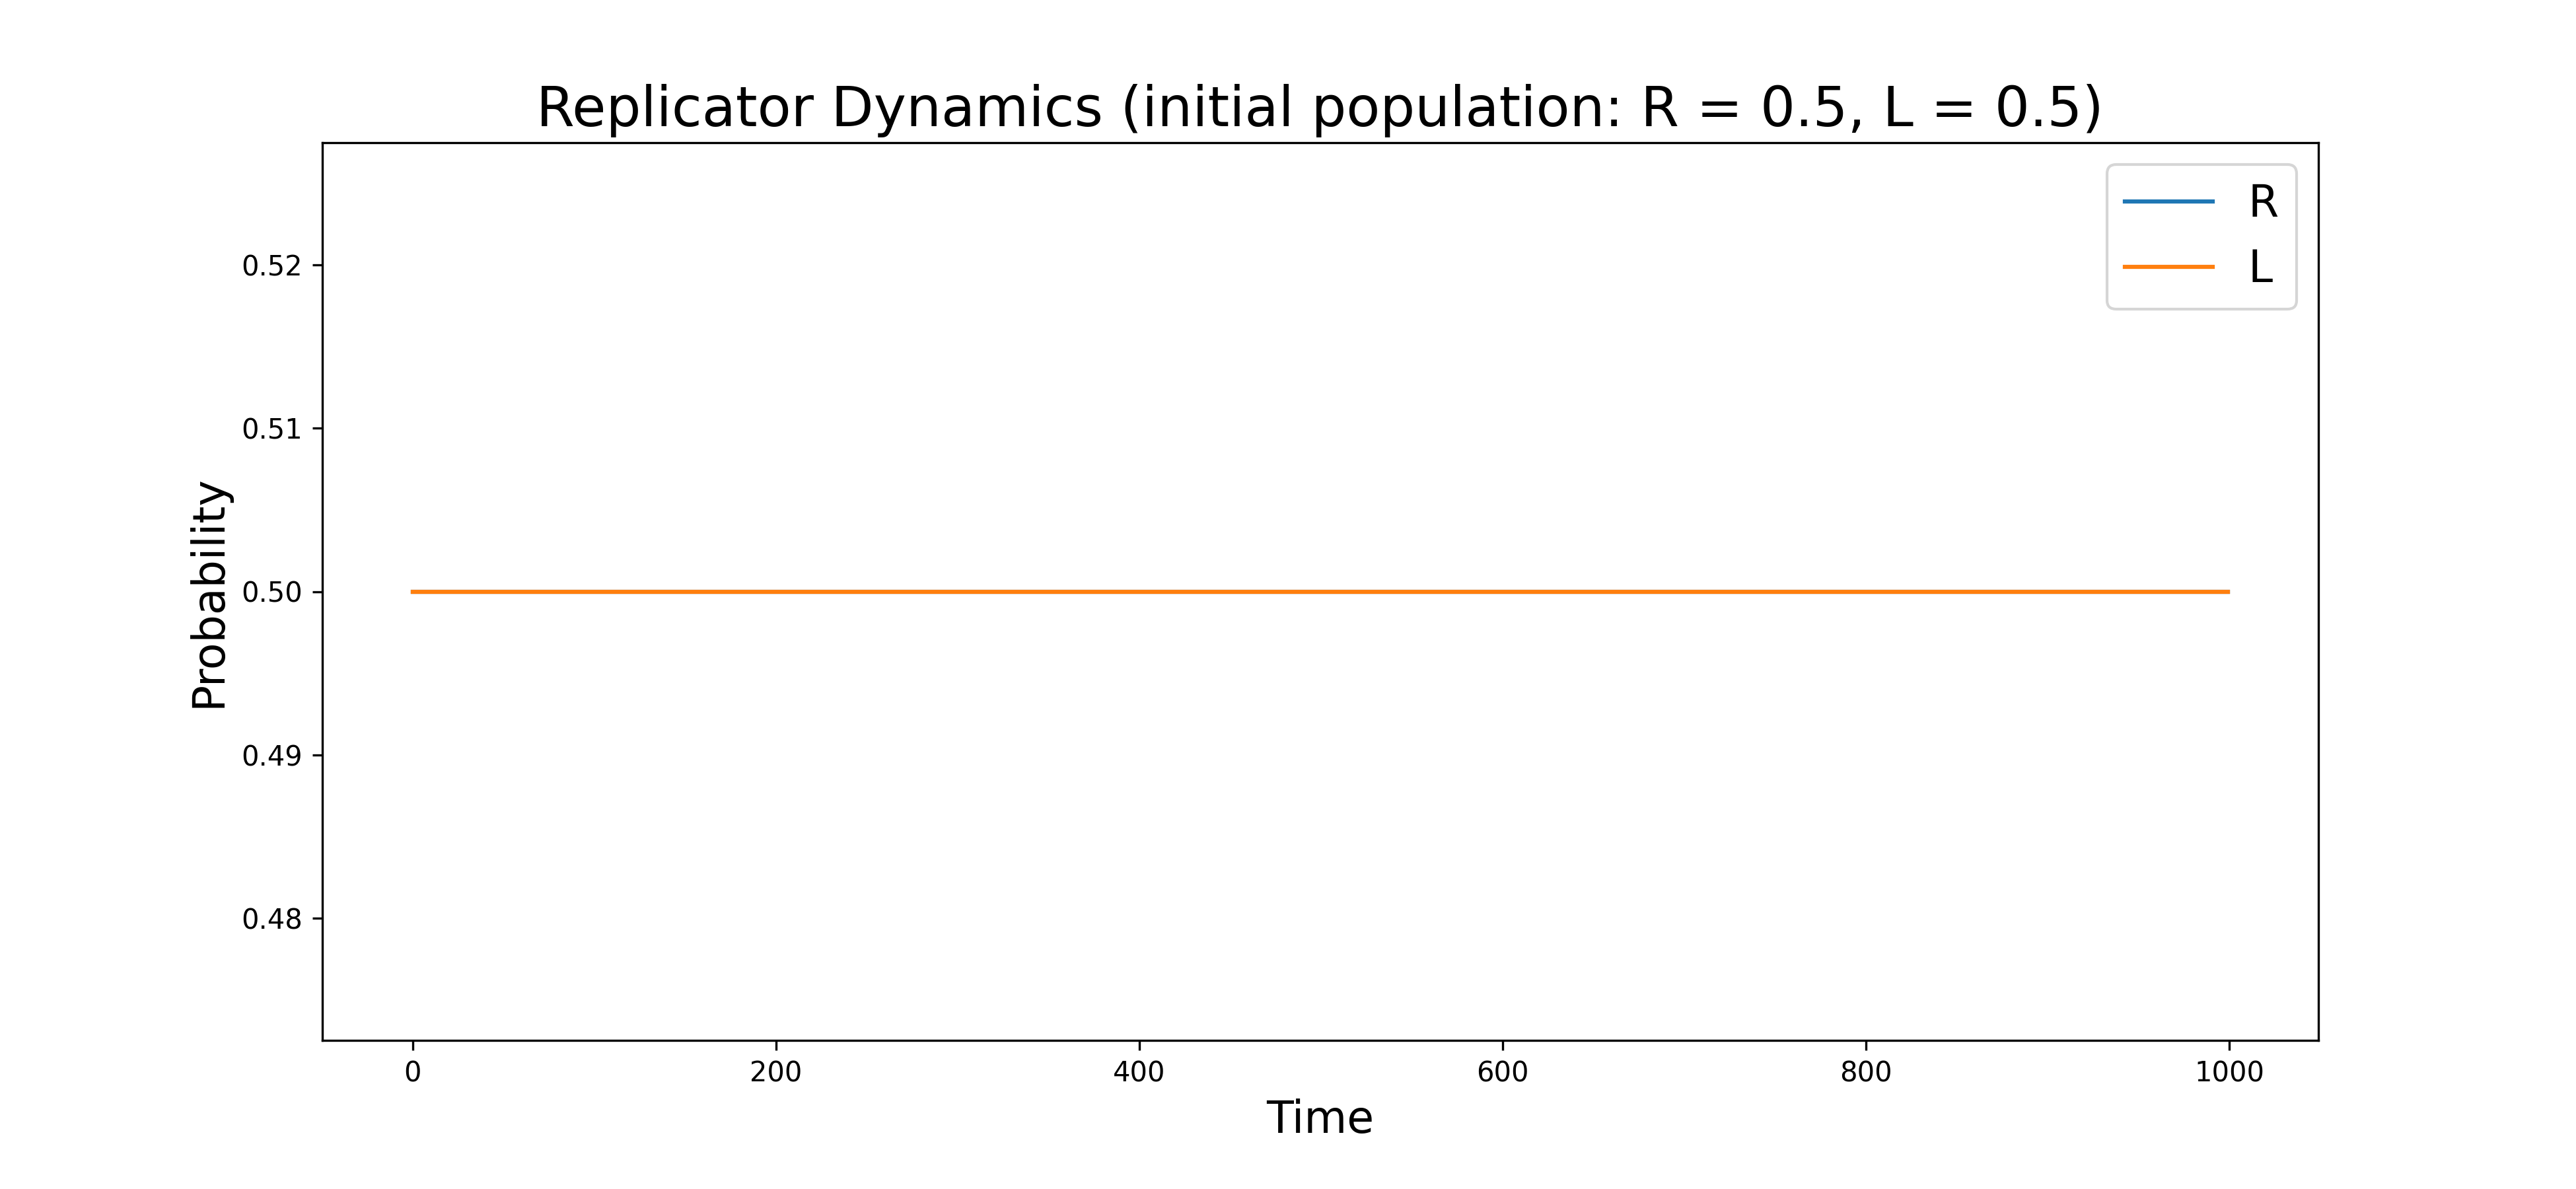
\includegraphics[width=\textwidth]{Bin/rps_ard/replicator_dynamics_example_1.png}
    }
    \only<3>{
        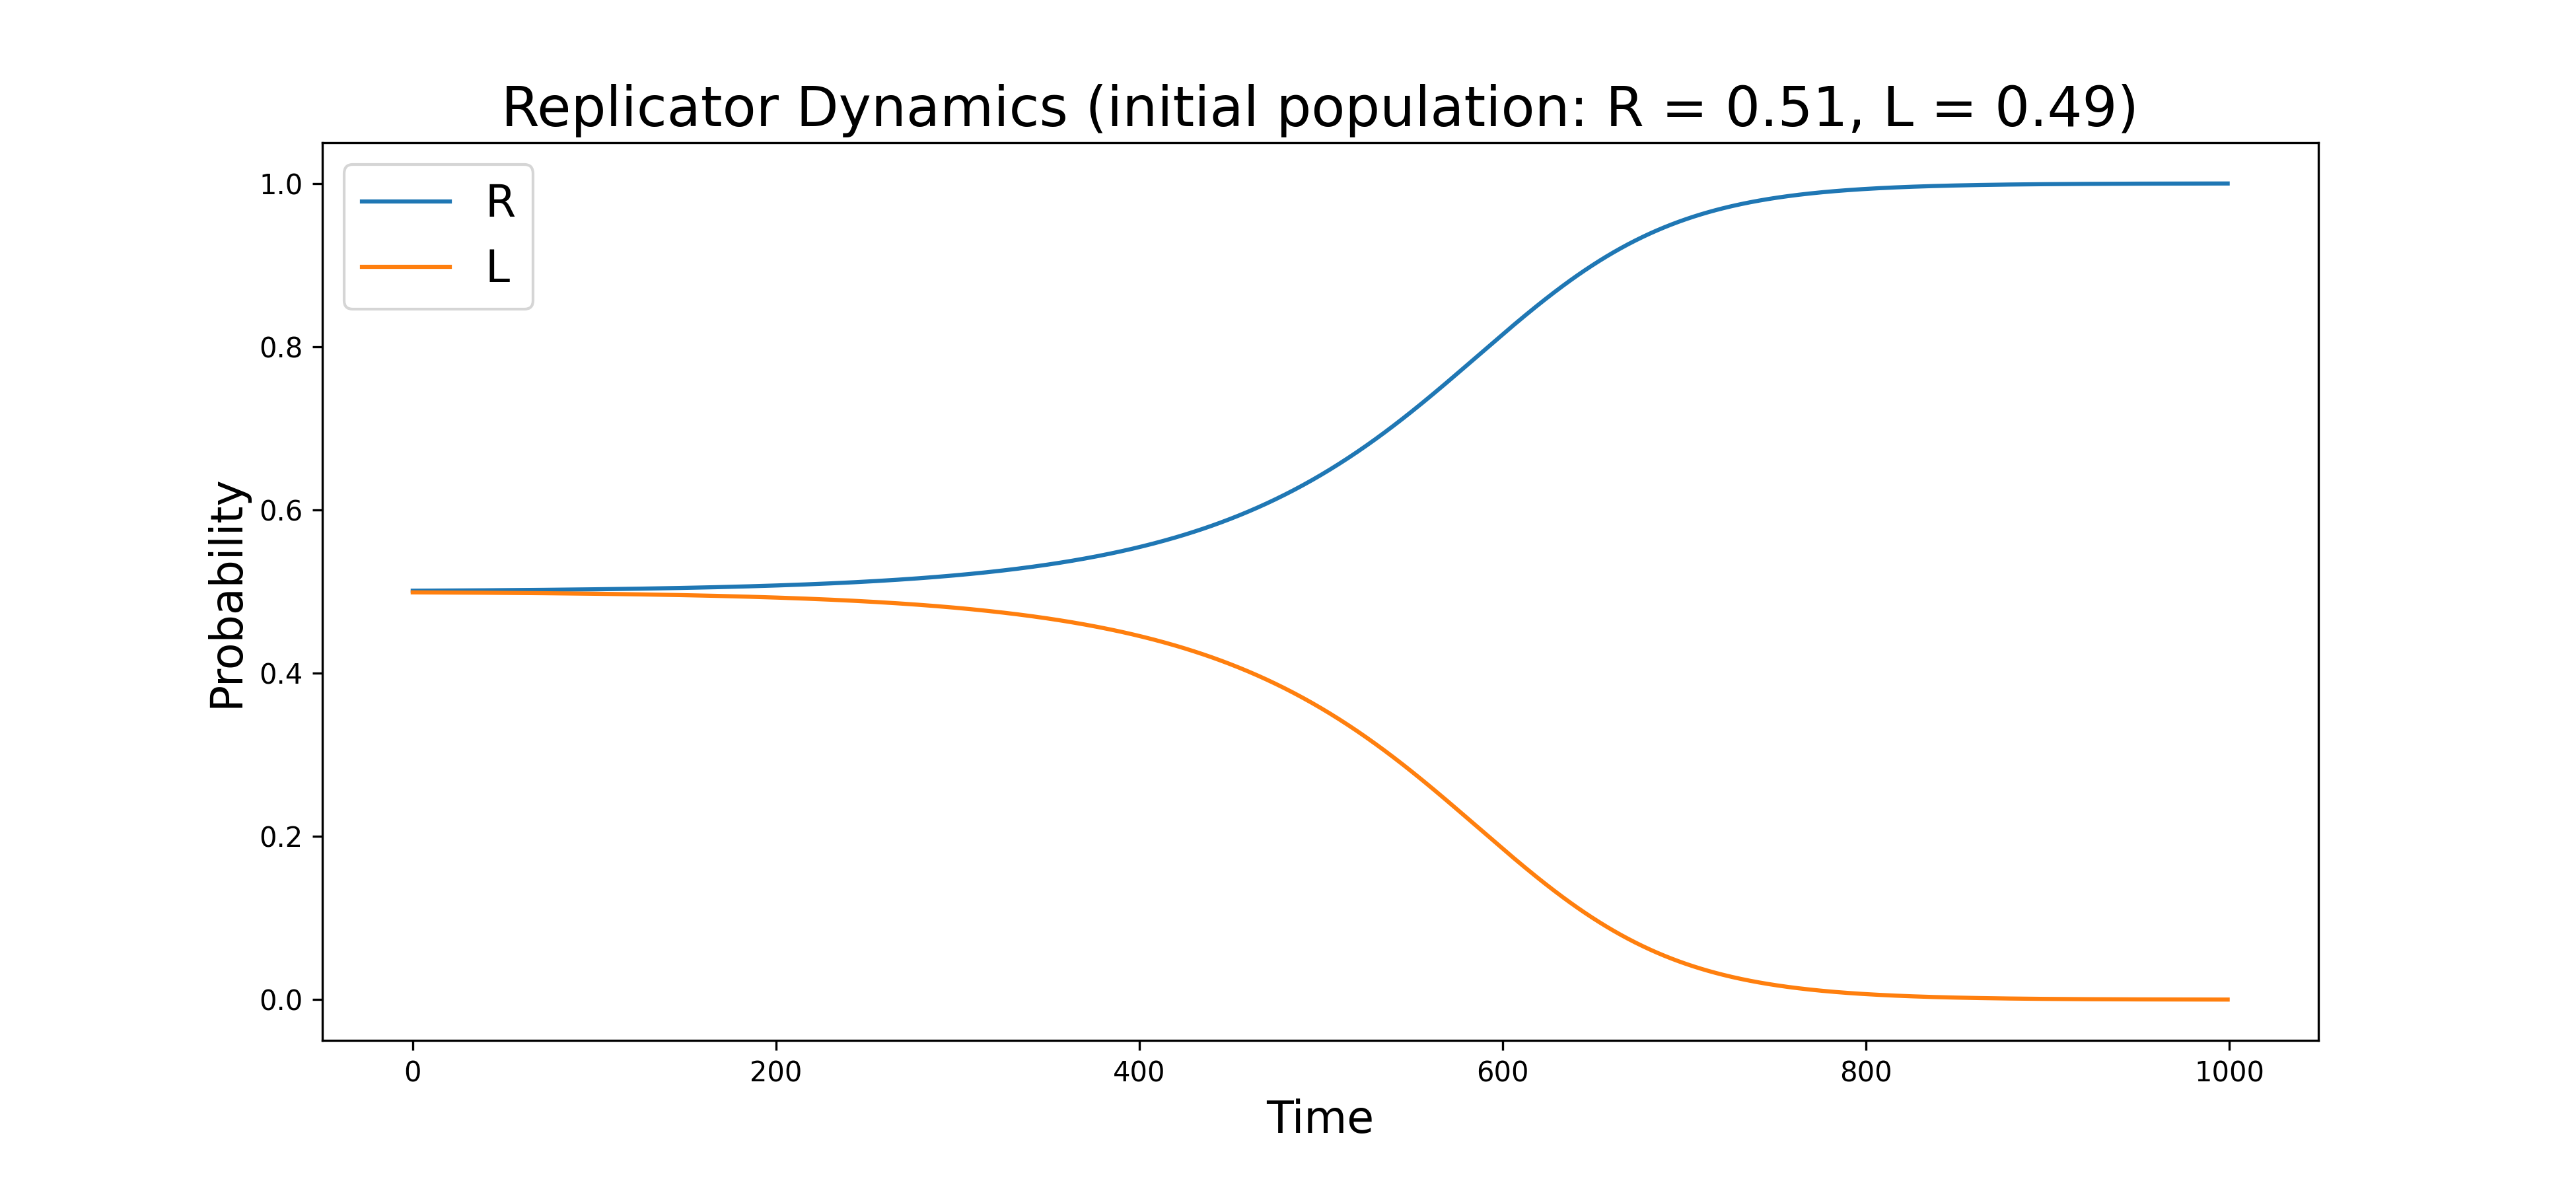
\includegraphics[width=\textwidth]{Bin/rps_ard/replicator_dynamics_example_2.png}
    }
    \only<4>{
        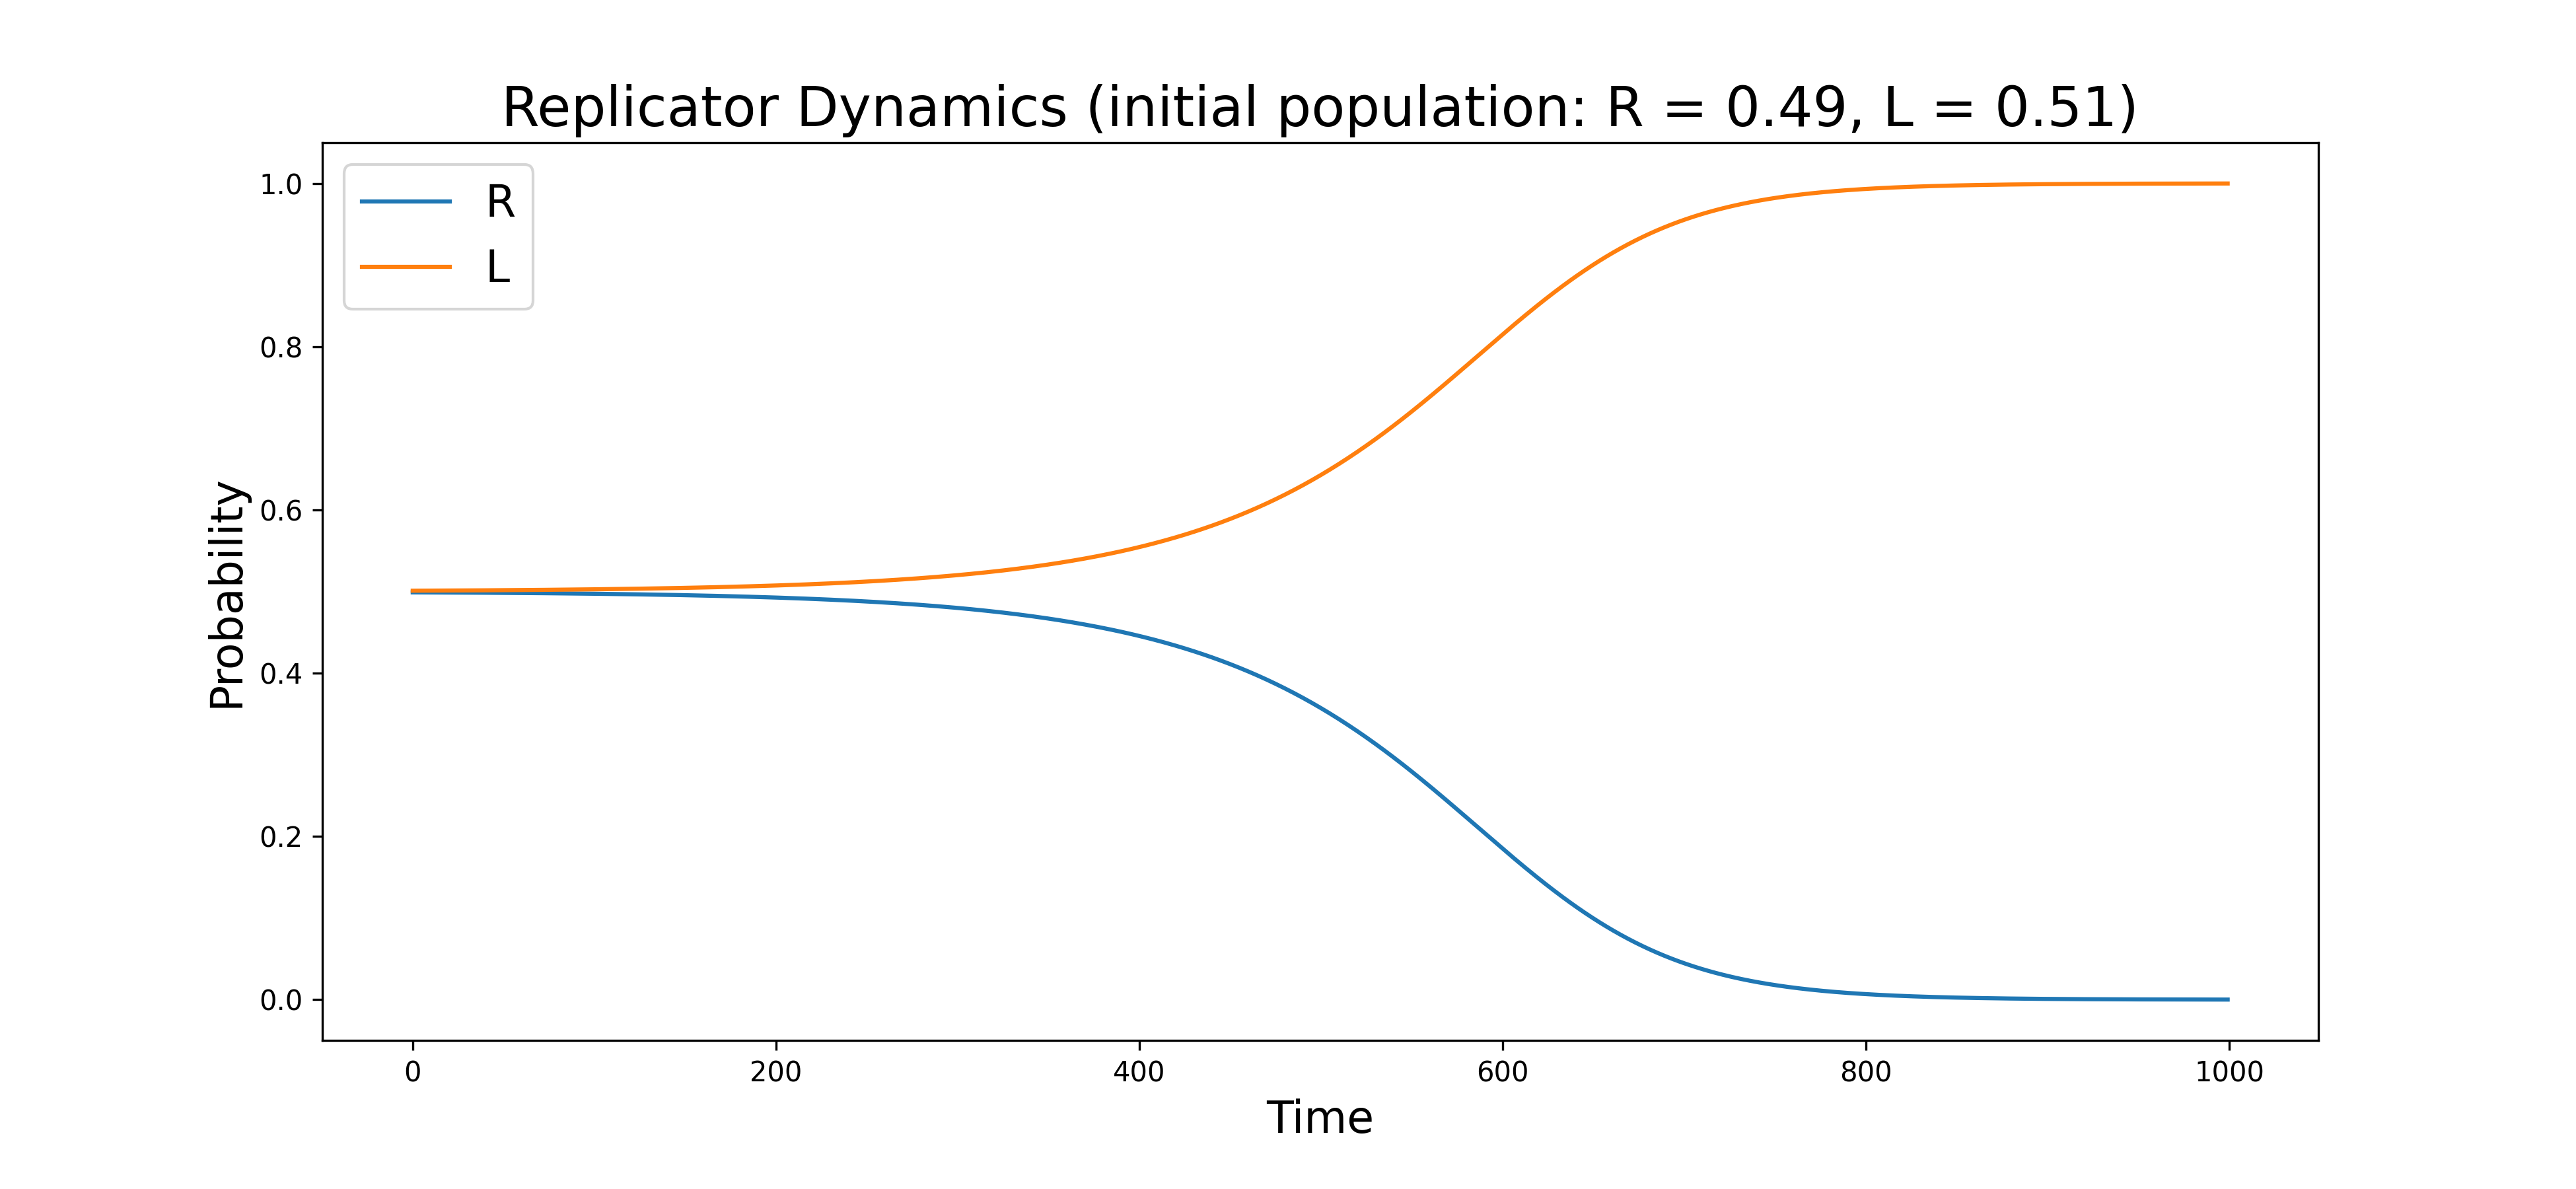
\includegraphics[width=\textwidth]{Bin/rps_ard/replicator_dynamics_example_3.png}
    }
    
\end{frame}



\begin{frame}
    \centering
    \Huge
    Evolutionary \\ Stable \\ Strategies
\end{frame}
